
%% bare_conf.tex
%% V1.3
%% 2007/01/11
%% by Michael Shell
%% See:
%% http://www.michaelshell.org/
%% for current contact information.
%%
%% This is a skeleton file demonstrating the use of IEEEtran.cls
%% (requires IEEEtran.cls version 1.7 or later) with an IEEE conference paper.
%%
%% Support sites:
%% http://www.michaelshell.org/tex/ieeetran/
%% http://www.ctan.org/tex-archive/macros/latex/contrib/IEEEtran/
%% and
%% http://www.ieee.org/

%%*************************************************************************
%% Legal Notice:
%% This code is offered as-is without any warranty either expressed or
%% implied; without even the implied warranty of MERCHANTABILITY or
%% FITNESS FOR A PARTICULAR PURPOSE! 
%% User assumes all risk.
%% In no event shall IEEE or any contributor to this code be liable for
%% any damages or losses, including, but not limited to, incidental,
%% consequential, or any other damages, resulting from the use or misuse
%% of any information contained here.
%%
%% All comments are the opinions of their respective authors and are not
%% necessarily endorsed by the IEEE.
%%
%% This work is distributed under the LaTeX Project Public License (LPPL)
%% ( http://www.latex-project.org/ ) version 1.3, and may be freely used,
%% distributed and modified. A copy of the LPPL, version 1.3, is included
%% in the base LaTeX documentation of all distributions of LaTeX released
%% 2003/12/01 or later.
%% Retain all contribution notices and credits.
%% ** Modified files should be clearly indicated as such, including  **
%% ** renaming them and changing author support contact information. **
%%
%% File list of work: IEEEtran.cls, IEEEtran_HOWTO.pdf, bare_adv.tex,
%%                    bare_conf.tex, bare_jrnl.tex, bare_jrnl_compsoc.tex
%%*************************************************************************

% *** Authors should verify (and, if needed, correct) their LaTeX system  ***
% *** with the testflow diagnostic prior to trusting their LaTeX platform ***
% *** with production work. IEEE's font choices can trigger bugs that do  ***
% *** not appear when using other class files.                            ***
% The testflow support page is at:
% http://www.michaelshell.org/tex/testflow/



% Note that the a4paper option is mainly intended so that authors in
% countries using A4 can easily print to A4 and see how their papers will
% look in print - the typesetting of the document will not typically be
% affected with changes in paper size (but the bottom and side margins will).
% Use the testflow package mentioned above to verify correct handling of
% both paper sizes by the user's LaTeX system.
%
% Also note that the "draftcls" or "draftclsnofoot", not "draft", option
% should be used if it is desired that the figures are to be displayed in
% draft mode.
%
\documentclass[conference]{IEEEtran}
% Add the compsoc option for Computer Society conferences.
%
% If IEEEtran.cls has not been installed into the LaTeX system files,
% manually specify the path to it like:
% \documentclass[conference]{../sty/IEEEtran}





% Some very useful LaTeX packages include:
% (uncomment the ones you want to load)


% *** MISC UTILITY PACKAGES ***
%
%\usepackage{ifpdf}
% Heiko Oberdiek's ifpdf.sty is very useful if you need conditional
% compilation based on whether the output is pdf or dvi.
% usage:
% \ifpdf
%   % pdf code
% \else
%   % dvi code
% \fi
% The latest version of ifpdf.sty can be obtained from:
% http://www.ctan.org/tex-archive/macros/latex/contrib/oberdiek/
% Also, note that IEEEtran.cls V1.7 and later provides a builtin
% \ifCLASSINFOpdf conditional that works the same way.
% When switching from latex to pdflatex and vice-versa, the compiler may
% have to be run twice to clear warning/error messages.






% *** CITATION PACKAGES ***
%
%\usepackage{cite}
% cite.sty was written by Donald Arseneau
% V1.6 and later of IEEEtran pre-defines the format of the cite.sty package
% \cite{} output to follow that of IEEE. Loading the cite package will
% result in citation numbers being automatically sorted and properly
% "compressed/ranged". e.g., [1], [9], [2], [7], [5], [6] without using
% cite.sty will become [1], [2], [5]--[7], [9] using cite.sty. cite.sty's
% \cite will automatically add leading space, if needed. Use cite.sty's
% noadjust option (cite.sty V3.8 and later) if you want to turn this off.
% cite.sty is already installed on most LaTeX systems. Be sure and use
% version 4.0 (2003-05-27) and later if using hyperref.sty. cite.sty does
% not currently provide for hyperlinked citations.
% The latest version can be obtained at:
% http://www.ctan.org/tex-archive/macros/latex/contrib/cite/
% The documentation is contained in the cite.sty file itself.






% *** GRAPHICS RELATED PACKAGES ***
%
\ifCLASSINFOpdf
  % \usepackage[pdftex]{graphicx}
  % declare the path(s) where your graphic files are
  % \graphicspath{{../pdf/}{../jpeg/}}
  % and their extensions so you won't have to specify these with
  % every instance of \includegraphics
  % \DeclareGraphicsExtensions{.pdf,.jpeg,.png}
\else
  % or other class option (dvipsone, dvipdf, if not using dvips). graphicx
  % will default to the driver specified in the system graphics.cfg if no
  % driver is specified.
  % \usepackage[dvips]{graphicx}
  % declare the path(s) where your graphic files are
  % \graphicspath{{../eps/}}
  % and their extensions so you won't have to specify these with
  % every instance of \includegraphics
  % \DeclareGraphicsExtensions{.eps}
\fi
% graphicx was written by David Carlisle and Sebastian Rahtz. It is
% required if you want graphics, photos, etc. graphicx.sty is already
% installed on most LaTeX systems. The latest version and documentation can
% be obtained at: 
% http://www.ctan.org/tex-archive/macros/latex/required/graphics/
% Another good source of documentation is "Using Imported Graphics in
% LaTeX2e" by Keith Reckdahl which can be found as epslatex.ps or
% epslatex.pdf at: http://www.ctan.org/tex-archive/info/
%
% latex, and pdflatex in dvi mode, support graphics in encapsulated
% postscript (.eps) format. pdflatex in pdf mode supports graphics
% in .pdf, .jpeg, .png and .mps (metapost) formats. Users should ensure
% that all non-photo figures use a vector format (.eps, .pdf, .mps) and
% not a bitmapped formats (.jpeg, .png). IEEE frowns on bitmapped formats
% which can result in "jaggedy"/blurry rendering of lines and letters as
% well as large increases in file sizes.
%
% You can find documentation about the pdfTeX application at:
% http://www.tug.org/applications/pdftex





% *** MATH PACKAGES ***
%
%\usepackage[cmex10]{amsmath}
% A popular package from the American Mathematical Society that provides
% many useful and powerful commands for dealing with mathematics. If using
% it, be sure to load this package with the cmex10 option to ensure that
% only type 1 fonts will utilized at all point sizes. Without this option,
% it is possible that some math symbols, particularly those within
% footnotes, will be rendered in bitmap form which will result in a
% document that can not be IEEE Xplore compliant!
%
% Also, note that the amsmath package sets \interdisplaylinepenalty to 10000
% thus preventing page breaks from occurring within multiline equations. Use:
%\interdisplaylinepenalty=2500
% after loading amsmath to restore such page breaks as IEEEtran.cls normally
% does. amsmath.sty is already installed on most LaTeX systems. The latest
% version and documentation can be obtained at:
% http://www.ctan.org/tex-archive/macros/latex/required/amslatex/math/





% *** SPECIALIZED LIST PACKAGES ***
%
%\usepackage{algorithmic}
% algorithmic.sty was written by Peter Williams and Rogerio Brito.
% This package provides an algorithmic environment fo describing algorithms.
% You can use the algorithmic environment in-text or within a figure
% environment to provide for a floating algorithm. Do NOT use the algorithm
% floating environment provided by algorithm.sty (by the same authors) or
% algorithm2e.sty (by Christophe Fiorio) as IEEE does not use dedicated
% algorithm float types and packages that provide these will not provide
% correct IEEE style captions. The latest version and documentation of
% algorithmic.sty can be obtained at:
% http://www.ctan.org/tex-archive/macros/latex/contrib/algorithms/
% There is also a support site at:
% http://algorithms.berlios.de/index.html
% Also of interest may be the (relatively newer and more customizable)
% algorithmicx.sty package by Szasz Janos:
% http://www.ctan.org/tex-archive/macros/latex/contrib/algorithmicx/




% *** ALIGNMENT PACKAGES ***
%
%\usepackage{array}
% Frank Mittelbach's and David Carlisle's array.sty patches and improves
% the standard LaTeX2e array and tabular environments to provide better
% appearance and additional user controls. As the default LaTeX2e table
% generation code is lacking to the point of almost being broken with
% respect to the quality of the end results, all users are strongly
% advised to use an enhanced (at the very least that provided by array.sty)
% set of table tools. array.sty is already installed on most systems. The
% latest version and documentation can be obtained at:
% http://www.ctan.org/tex-archive/macros/latex/required/tools/


%\usepackage{mdwmath}
%\usepackage{mdwtab}
% Also highly recommended is Mark Wooding's extremely powerful MDW tools,
% especially mdwmath.sty and mdwtab.sty which are used to format equations
% and tables, respectively. The MDWtools set is already installed on most
% LaTeX systems. The lastest version and documentation is available at:
% http://www.ctan.org/tex-archive/macros/latex/contrib/mdwtools/


% IEEEtran contains the IEEEeqnarray family of commands that can be used to
% generate multiline equations as well as matrices, tables, etc., of high
% quality.


%\usepackage{eqparbox}
% Also of notable interest is Scott Pakin's eqparbox package for creating
% (automatically sized) equal width boxes - aka "natural width parboxes".
% Available at:
% http://www.ctan.org/tex-archive/macros/latex/contrib/eqparbox/





% *** SUBFIGURE PACKAGES ***
%\usepackage[tight,footnotesize]{subfigure}
% subfigure.sty was written by Steven Douglas Cochran. This package makes it
% easy to put subfigures in your figures. e.g., "Figure 1a and 1b". For IEEE
% work, it is a good idea to load it with the tight package option to reduce
% the amount of white space around the subfigures. subfigure.sty is already
% installed on most LaTeX systems. The latest version and documentation can
% be obtained at:
% http://www.ctan.org/tex-archive/obsolete/macros/latex/contrib/subfigure/
% subfigure.sty has been superceeded by subfig.sty.



%\usepackage[caption=false]{caption}
%\usepackage[font=footnotesize]{subfig}
% subfig.sty, also written by Steven Douglas Cochran, is the modern
% replacement for subfigure.sty. However, subfig.sty requires and
% automatically loads Axel Sommerfeldt's caption.sty which will override
% IEEEtran.cls handling of captions and this will result in nonIEEE style
% figure/table captions. To prevent this problem, be sure and preload
% caption.sty with its "caption=false" package option. This is will preserve
% IEEEtran.cls handing of captions. Version 1.3 (2005/06/28) and later 
% (recommended due to many improvements over 1.2) of subfig.sty supports
% the caption=false option directly:
%\usepackage[caption=false,font=footnotesize]{subfig}
%
% The latest version and documentation can be obtained at:
% http://www.ctan.org/tex-archive/macros/latex/contrib/subfig/
% The latest version and documentation of caption.sty can be obtained at:
% http://www.ctan.org/tex-archive/macros/latex/contrib/caption/




% *** FLOAT PACKAGES ***
%
%\usepackage{fixltx2e}
% fixltx2e, the successor to the earlier fix2col.sty, was written by
% Frank Mittelbach and David Carlisle. This package corrects a few problems
% in the LaTeX2e kernel, the most notable of which is that in current
% LaTeX2e releases, the ordering of single and double column floats is not
% guaranteed to be preserved. Thus, an unpatched LaTeX2e can allow a
% single column figure to be placed prior to an earlier double column
% figure. The latest version and documentation can be found at:
% http://www.ctan.org/tex-archive/macros/latex/base/



%\usepackage{stfloats}
% stfloats.sty was written by Sigitas Tolusis. This package gives LaTeX2e
% the ability to do double column floats at the bottom of the page as well
% as the top. (e.g., "\begin{figure*}[!b]" is not normally possible in
% LaTeX2e). It also provides a command:
%\fnbelowfloat
% to enable the placement of footnotes below bottom floats (the standard
% LaTeX2e kernel puts them above bottom floats). This is an invasive package
% which rewrites many portions of the LaTeX2e float routines. It may not work
% with other packages that modify the LaTeX2e float routines. The latest
% version and documentation can be obtained at:
% http://www.ctan.org/tex-archive/macros/latex/contrib/sttools/
% Documentation is contained in the stfloats.sty comments as well as in the
% presfull.pdf file. Do not use the stfloats baselinefloat ability as IEEE
% does not allow \baselineskip to stretch. Authors submitting work to the
% IEEE should note that IEEE rarely uses double column equations and
% that authors should try to avoid such use. Do not be tempted to use the
% cuted.sty or midfloat.sty packages (also by Sigitas Tolusis) as IEEE does
% not format its papers in such ways.





% *** PDF, URL AND HYPERLINK PACKAGES ***
%
%\usepackage{url}
% url.sty was written by Donald Arseneau. It provides better support for
% handling and breaking URLs. url.sty is already installed on most LaTeX
% systems. The latest version can be obtained at:
% http://www.ctan.org/tex-archive/macros/latex/contrib/misc/
% Read the url.sty source comments for usage information. Basically,
% \url{my_url_here}.





% *** Do not adjust lengths that control margins, column widths, etc. ***
% *** Do not use packages that alter fonts (such as pslatex).         ***
% There should be no need to do such things with IEEEtran.cls V1.6 and later.
% (Unless specifically asked to do so by the journal or conference you plan
% to submit to, of course. )

\usepackage{url}
\usepackage{amsmath}
\usepackage{xcolor}
\usepackage{comment}

\usepackage[english]{babel}
\usepackage{graphicx}

\newcommand\jedit[1]{\textcolor{red}{Jim -- #1}}
\newcommand\vedit[1]{\textcolor{cyan}{Vijay -- #1}}
\newcommand\redit[1]{\textcolor{blue}{Ross -- #1}}
\newcommand\sedit[1]{\textcolor{magenta}{Sean -- #1}}
\newcommand\outlineedit[1]{\textcolor{green}{}}
\DeclareMathOperator*{\argmax}{arg\,max}
\DeclareMathOperator*{\argmin}{arg\,min}

% correct bad hyphenation here
\hyphenation{op-tical net-works semi-conduc-tor}


\begin{document}
%
% paper title
% can use linebreaks \\ within to get better formatting as desired
\title{Setting Password Policies Using Cognitive Behavioral Agent-Based Modeling\\[.75ex] 
%  {\normalfont\large 
%	Vijay Kothari\IEEEauthorrefmark{1},
%	Jim Blythe\IEEEauthorrefmark{2},
%	Ross Koppel\IEEEauthorrefmark{3}, and
%	Sean Smith\IEEEauthorrefmark{1}
%  }\\[-1.5ex]
}

% sws: fixed author alignment, via http://tex.aspcode.net/view/635399273629833626287708/multiple-authors-with-multiple-affiliations

% author names and affiliations
% use a multiple column layout for up to three different
% affiliations
%\author{\IEEEauthorblockA{\IEEEauthorrefmark{1}Department of Computer Science\\
%Dartmouth College\\
%\{vijayk,sws\}@cs.dartmouth.edu}\and
%\IEEEauthorblockA{\IEEEauthorrefmark{2}Information Sciences Institute\\
%University of Southern California\\
%blythe@isi.edu}\and
%\IEEEauthorblockA{\IEEEauthorrefmark{3}Department of Sociology\\
%University of Pennsylvania\\
%rkoppel@sas.upenn.edu}}


% conference papers do not typically use \thanks and this command
% is locked out in conference mode. If really needed, such as for
% the acknowledgment of grants, issue a \IEEEoverridecommandlockouts
% after \documentclass

% for over three affiliations, or if they all won't fit within the width
% of the page, use this alternative format:
% 
%\author{\IEEEauthorblockN{Michael Shell\IEEEauthorrefmark{1},
%Homer Simpson\IEEEauthorrefmark{2},
%James Kirk\IEEEauthorrefmark{3}, 
%Montgomery Scott\IEEEauthorrefmark{3} and
%Eldon Tyrell\IEEEauthorrefmark{4}}
%\IEEEauthorblockA{\IEEEauthorrefmark{1}School of Electrical and Computer Engineering\\
%Georgia Institute of Technology,
%Atlanta, Georgia 30332--0250\\ Email: see http://www.michaelshell.org/contact.html}
%\IEEEauthorblockA{\IEEEauthorrefmark{2}Twentieth Century Fox, Springfield, USA\\
%Email: homer@thesimpsons.com}
%\IEEEauthorblockA{\IEEEauthorrefmark{3}Starfleet Academy, San Francisco, California 96678-2391\\
%Telephone: (800) 555--1212, Fax: (888) 555--1212}
%\IEEEauthorblockA{\IEEEauthorrefmark{4}Tyrell Inc., 123 Replicant Street, Los Angeles, California 90210--4321}}




% use for special paper notices
%\IEEEspecialpapernotice{(Invited Paper)}




% make the title area
\maketitle


\begin{abstract}
%\boldmath
Agent-based modeling can serve as a valuable asset to security
personnel who wish to better understand the security landscape within
their organization, especially as it relates to user behavior and
circumvention. In this paper, we argue in favor of agent-based
modeling for usable security, report on our work on developing an
agent-based model for a password management scenario, and provide
directions for future work.
\end{abstract}
% IEEEtran.cls defaults to using nonbold math in the Abstract.
% This preserves the distinction between vectors and scalars. However,
% if the conference you are submitting to favors bold math in the abstract,
% then you can use LaTeX's standard command \boldmath at the very start
% of the abstract to achieve this. Many IEEE journals/conferences frown on
% math in the abstract anyway.

% no keywords




% For peer review papers, you can put extra information on the cover
% page as needed:
% \ifCLASSOPTIONpeerreview
% \begin{center} \bfseries EDICS Category: 3-BBND \end{center}
% \fi
%
% For peerreview papers, this IEEEtran command inserts a page break and
% creates the second title. It will be ignored for other modes.
\IEEEpeerreviewmaketitle

\newcommand{\dash}{{\sc dash}}

\section{Introduction}
\label{Introduction}
% no \IEEEPARstart

Agent-based models incorporating user behavior, emotion, and 
cognition can serve as valuable tools that assist computer security 
personnel design, implement, and maintain security systems, 
devise security policies, and employ security practices that 
are congruent with security and other organizational objectives.

Indeed, as the current state of security practice indicates, we need 
these sorts of tools. Our interviews, surveys, and observations reflect many 
examples where security fails to accommodate users. Such 
mismatches between user needs and security policies and 
mechanisms often induce circumvention, thereby undermining 
overall objectives. Even if one could design adequate security
policies and mechanisms a priori, the dynamic nature of software
systems, user needs, and organizational and environmental 
changes would necessitate frequent readjustments. 
Consequently, we need tools that allow us to better understand 
computer security's costs, common perceptions and misperceptions, 
side effects, and interactions.

\dash\ \cite{blythe2012implementing, blythe2012dual}, an agent-based 
simulation framework that supports the dual-process model of 
cognition, reactive planning, modeling of human deficiencies 
(e.g., fatigue, frustration), and multi-agent interactions, enables us to 
create such tools. In \dash, 
users are represented as agents with weighted goals, plans to 
achieve those goals, attributes, knowledge, and abilities. These 
agents use mental models and have perceptions of the world that 
often depart from reality. In accordance with their mental models, 
they take actions, observe and interpret events, and communicate. 
They dynamically compute and recompute goals and the plans 
they use to achieve them. \dash\ models may better enable 
security personnel to (a) identify weaknesses in security 
policies and mechanisms, e.g., workflow impediments that 
prompt user circumvention, (b) estimate the likelihood of user 
engagement in workarounds, (c) gauge the number of 
inescapable security infractions from policy-workflow 
mismatches, (d) estimate the values of security and 
organizational objective functions, (e) test the accuracy of 
proxy security measures, and (f) measure the impacts that shifts 
in the environment have on security. A cognitive and 
behavioral-centric approach to modeling can 
provide insights into the effectiveness of informing users of 
practical needs for security, implementing a feedback loop, 
imposing more stringent policies or harsher penalties for 
circumvention, and more.

Agent-based modeling is particularly enlightening in scenarios 
where security in practice radically differs from security in 
the abstract, where it's extraordinarily challenging to anticipate 
how emotions, cognitive biases, and other human deficiencies 
may affect user behavior. Indeed, in order to get security right it is 
critical that we understand how users interact with our systems.
And we must adapt our systems to our users (and not 
expect our users to adapt to our systems!) so as to induce ``good'' 
behavior \cite{blythe2013circumvention, adams1999users}. In previous work 
\cite{kothari2014agent} we discussed the potential for agent-based 
models to be applied to prediction of human circumvention of security, 
relayed an anecdote regarding timeouts in a medical setting, 
explained our preliminary work, and discussed our future directions 
for building such models. In this paper, we follow up on this 
work by detailing our progress on modeling the password 
management scenario.

The password management scenario involves establishing password
polices for an enterprise. In theory, having a policy that requires users 
to use strong passwords, to never write them down, and to never 
reuse them across sites would improve security.  In practice, users commonly 
circumvent password policies due to perceived cognitive limitations, 
fatigue, frustration, and work culture. Password choices and password 
management practices for one service may affect the choices and 
practices for another, making the services interdependent. By applying 
agent-based models, security personnel can better understand this 
complex environment, estimate measures of aggregate security that 
incorporate circumventions, risks, and costs, and ultimately make 
better decisions.

\begin{comment}
Our first scenario focuses on choosing a timeout threshold 
for de-authentication in hospital settings, where clinicians share 
computers. In theory, timed auto-logout should reduce both the 
security risks of unattended machines with active sessions and 
the healthcare risks of clinicians inadvertently using the wrong 
session. However, in practice, clinicians must log in up to 200 
times daily, taking, by some estimates, an eighth of their time; 
so, they find workarounds to defeat auto-logout mechanisms. 
Too long of a threshold weakens security by exposing 
sessions, while too short of a threshold  weakens security
by promoting circumvention. An optimal threshold
depends on a complex mix of human-centric factors. Both short 
and long timeouts can induce frustration and lead to user 
circumvention. But the underlying causes and repercussions 
on healthcare may be very different. Applying agent-based
simulations tailored to the environment and user subpopulations, 
we aim to predict the organizational impact of various timeout
thresholds, derive an optimal threshold, and suggest alternative 
timeout mechanisms.
\end{comment}

This paper is structured as follows. In Section \ref{dash}, we 
introduce the \dash\ modeling framework. in Section \ref{password} 
we investigate the password modeling scenario, detail our \dash\ 
modeling work, and remark on how this model may be used to 
provide security personnel with valuable insights that guide them 
to make better security decisions. In Section \ref{future_work} we 
discuss future work including the autologout scenario. In Section 
\ref{conclusion} we draw conclusions.

\section{The DASH agent modeling platform}
\label{dash}

The {\sc dash} agent modeling platform provides a framework 
and a set of capabilities for modeling human behavior 
\cite{blythe2012implementing}, designed to capture observations 
from human-centered security experiments, e.g. 
\cite{dhamija2006phishing}. In order to model human 
task-oriented behavior, which is both goal-directed and responsive 
to changes in the environment, {\sc dash} includes a reactive 
planning framework that re-assesses goal weights and plans after 
receiving input after an action \cite{bratman1987intention}. In 
order to model deliberative behavior, {\sc  dash} includes an 
implementation of mental models following the approach of 
Johnson-Laird and others \cite{johnson1986mental} and a simple 
framework for evaluating costs and benefits of alternative worlds. 
This approach adopts the view that users follow essentially rational behavior 
when making decisions about on-line actions including security, 
but typically have an incomplete or incorrect model of the security 
landscape. 

In order to model bounded attention that affects human 
decision-making, particularly under stress or cognitive load, 
{\sc dash} includes a dual-process framework 
\cite{stanovich2000advancing} in which two modules provide 
alternative suggestions for the agent's next action. The first is a 
deliberative system that uses the mechanisms for planning and 
mental models to arrive at a decision, and the second is a 
stimulus-driven system that matches surface properties of a 
situation to find an answer. Once an agent has experience in a 
domain, the stimulus system provides good answers most of the 
time while an inexperienced agent may need to fall back on 
deliberative reasoning more often. Under stress, time pressure, 
or cognitive load, the deliberative system may not complete, or 
the stimulus system may gain increased weight, leading to 
impulsive behavior that may not be correct.

Other cognitive architectures such as SOAR \cite{laird1987soar} or 
ACT-R \cite{anderson1993problem} provide many of the same 
behaviors. One distinguishing factor of {\sc dash} is that its stimulus 
system is not related to the deliberative system by a compilation 
learning process and can often produce results that differ 
qualitatively rather than in terms of speed. {\sc dash} also provides 
support for mental models and tradeoff analysis as more 
fundamental components.

\outlineedit{Here, we provide an overview of our approach. We are still working 
on the simulation, but this is what we are currently aspiring to; our 
approach may change in the future.

Agents correspond to clinicians who go about their jobs. They try 
to optimize some objective function incorporating aspects of patient 
care, security compliance, and more. However, they are also 
susceptible to fatigue and frustration, which may cloud their rational 
system 2 thought. Moreover, they are part of a group. A clinician will 
frequently interact with other clinicians and patients, which 
influences their own thought processes. Beliefs, attitudes, and 
behaviors spread amongst subpopulations of clinicians, as do 
notions of acceptability of circumvention. Agents are more inclined 
to follow security policies they deem rational, security-minded, and 
easily adoptable over ones that seem irrational and get in the way 
of patient care.

Agents regularly log in to and log out of machines, which takes its 
toll. While aware of patient data risks, they also have limited 
resources to expend including time and cognitive 
resources (e.g., being logged out of a session may lead to 
inaccurate charting). 

Some of the modeling parameters that we hope to capture in our 
simulation are the number of agents, diversity and subpopulations 
of agents, de-authentication mechanisms and associated 
parameters (e.g., the time-out threshold for fixed timeouts), 
security policies, and agent attributes.}

\outlineedit{Suggested outline: discussion of the observation of the
  workaround and how it was a surprise to the developers. This
  illustrates that it is essential, not just optional, to find
  solutions that make sense in the context of an enterprise workflow:
  they are the only solutions that will be used. It is usually
  impractical for developers to test alternative approaches for
  security technology and policy in each potential enterprise, and
  multi-agent simulations may play an important role in predicting the
  stress points of a candidate implementation and suggesting which
  approaches are more appropriate for a location.  It is not necessary
  to predict an inventive workaround such as the plastic cup used here
  in order to help find better solutions, but only to predict where
  difficulties introduced by a potential approach might encourage
  people to seek a workaround.

In the case of auto-logouts, three main forces come into
  play. First, the use of shared workstations for a task that involves
  frequently moving leads to the possibility of using another's
  credentials, inadvertently or not. Second the nature of the task
  (prescribing medication and noting its delivery) makes this
  possibility dangerous. Third, the frequency of leaving and returning
  coupled with the time spent logging in multiple times makes the
  auto-logout solution a painful one in this scenario.

Using simulation we can explore the factors that lead to the
  danger of using a terminal with someone else logged in: the
  likelihood of this depends on the number of agents, the number of
  workstations and the dynamic nature of the task, while its danger
  depends on the kinds of tasks being performed. We can also explore
  the costs to workers of using different kinds of solutions, for
  example auto-logout versus authentication challenges after a period
  of inactivity that may be quicker to take effect than a full login,
  or detecting tasks that are not in the flow of the current task for
  the terminal in order to warn users that they may be on a terminal
  use by another, and warning about logout while other terminals in
  the cluster are free. For a range of tasks it may well be possible
  to predict whether the worker needs to return to complete a session
  or if it is conceptually completed, and apply different policies
  based on this. We show simulations below that can contrast these
  approaches in terms of reduced danger compared to additional cost
  for workers, under a range of assumptions about the location.}

\section{The Password Management Scenario: Security Dependencies
  Introduced by Workarounds}
\label{password}

\subsection{Prelminaries}

In terms of usability and security, many consider passwords a failure. 
Users are notorious for choosing weak passwords 
\cite{spafford1992opus}. In an effort to mitigate the security risks 
linked to weak passwords, many services now require users to 
choose passwords that satisfy complex password composition rules. 
Unfortunately, this brings with it a slew of other security challenges 
\cite{blythe2013circumvention, florencio2014password, gaw2006password, adams1999users}. 
Users who are unable to cope with the increased cognitive demands 
of having to remember dozens of passwords resort to circumventing 
password policies and employing poor password management 
strategies; they write passwords down on Post-it notes, reuse 
passwords across multiple services with little or no variation, and 
leave passwords in plaintext files on their computers. However, 
perceived cognitive limitations are not the only impetus for user 
circumvention of password policies. In some domains, users need 
to share information with others who have different access rights 
than themselves, but the ``proper'' channel for information sharing 
is slow and inefficient. So, they share passwords instead 
{\cite{blythe2013circumvention}.

Services are culpable too. Some services effectively discourage 
strong passwords by setting low ceilings on password length, 
disallowing special characters, using easily guessable security 
questions, and assigning default passwords that are often left 
unchanged. Others impose excessive 
password complexity requirements and require frequent 
password resets, which further incentivizes users to circumvent. 
In recent years, 
many services have also been the target of massive password 
breaches; in some cases, they have even exposed passwords to 
malicious actors in cleartext. Moreover, due to password reuse, 
risks associated with poor password practices are not confined 
to those services that are lax about password security. That is, 
the security of even those services that make good efforts to 
secure user passwords can easily be compromised by 
vulnerabilities on other sites \cite{ives2004domino}.

While tremendous effort has been spent on trying to replace 
passwords, it has been met with questionable success. Bonneau 
et al \cite{bonneau2012quest} compared passwords to other 
authentication schemes in three domains: usability, deployability, 
and security. They showed that no alternative authentication 
scheme dominates passwords.

In short, passwords pose numerous memorability and usability 
challenges that frequently manifest in user circumvention. They 
pose confidentiality, risk mitigation, and public perception 
challenges for services-- even those services that take great 
efforts to secure password content. And they are not going 
away any time soon. This motivates the need for better 
techniques to both assess and mitigate costs and risks 
associated with password policies.

Numerous recent studies have looked into password modeling.  Shay et
al \cite{shay2007password} developed a simulation for understanding
the effectiveness of password policies. Choong
\cite{choong2014cognitive} proposed a user-centric
cognitive-behavioral framework for the password management lifecycle,
from password creation to password reset. SimPass is a highly
configurable agent-based model for measuring the efficacy of password
policies \cite{renaud2013simpass}. Our work is similar to SimPass in
that we've developed a password simulation with a number of knobs
that can be adjusted to measure aggregate security associated with
password policies under different circumstances. Whereas SimPass 
employs numerous parameters to better understand password 
management scenarios with minimal assumptions, we adopt the view 
that many of these parameters cannot be known, nor do they need to be 
known, \textit{a priori} to have a useful predictive model. Our simulation 
instead relies on only a small number of parameters and employs 
numerous underlying models, esp. those related to cognition and behavior. 
For example, there exist models for cognitive burden associated with 
passwords and password recall. The flip-side is that this approach 
necessitates us making more assumptions.

\subsection{Simulation Details}

\vedit{I'm not satisfied with this section. I'd like to rework it a bit}

In our simulation, agents create accounts for services, sign 
in to accounts, and sign out of accounts. The actions are
supported via simple underlying models for username and 
password recall and cognitive burden.

First, we discuss the model for password recall. For the rest 
of this discussion, we limit ourselves to passwords; a similar 
model exists for usernames. $V_{S, P}$  denotes the strength 
value for password $P$ on service $S$. When an agent attempts 
to sign in to a service, the password strength values associated with 
that service determine whether or not she recalls a password; and, 
if she does recall a password, it further determines which 
password she recalls.

We now discuss how the cognitive burden associated with 
usernames and passwords is calculated. As before, we limit 
our discussion to passwords. The model uses a generalization 
of the Levenshtein distance to sets. It make use of an openly 
available Prolog implementation of Levenshtein distance \cite{levdist}. 
The Levenshtein distance between a string $S_1$ and $S_2$ is the 
minimum number of character insertions, deletions, and substitutions 
required to convert $S_1$ into $S_2$. For set $S$, define the 
Levenshtein measure $L(S)$ to be the least weight tree $T$ that has 
vertex set $S \cup \{\epsilon\}$ and edge set $E$ where each edge 
$e = (v_1, v_2)$ has weight $w(v_1, v_2) = Lev(v_1, v_2)$. Here, 
$\epsilon$ denotes the empty string and $Lev(v_1, v_2)$ is the 
Levenshtein distance between $v_1$ and $v_2$. The cognitive 
burden of a set $S_P$ of passwords in our simulation is approximately 
$L(S_P)$. There is also a small cost associated with mapping 
passwords to services in memory. We very roughly approximate this 
by including an additive factor of 1 for each service that has a 
corresponding password that is in the agent's memory.

To assess the risk of password compromise, we consider three attack 
vectors. The first is a direct attack in which the attacker either exploits a 
service vulnerability or guesses the password. This is a function of a raw 
password strength function that maps passwords to strength values. The 
second is an attack by which a malicious user sees the agent's password 
written down and uses it to access the agent's account. The risk for this 
attack equals a specified model parameter if the password has been written 
down; else, it is 0. The last attack is an indirect attack by which, using 
one of the previously mentioned attacks, the attacker discovers the 
agent's password for another site; and then, she uses that password 
to log in to the target service. The risk of this attack is one minus the 
probability of being safe from indirect attacks, where the probability 
of being safe is the product of probabilities of being safe from indirect 
attacks from each service. The probability that a service $S$ is safe 
from an indirect attack through $S'$ is the product of a specified 
parameter with the probability that $S'$ is not compromised by a direct 
attack. We refer to the average value for this security measure over all 
services to be $M$.

Though flawed, we believe these models serve as a reasonable 
first approximation. We aspire to iteratively incorporate recent models 
and bounds (e.g., Flor\^{e}ncio et al \cite{florencio2014password} provide 
bounds on cognitive burden) into our simulation in the near future.

During account creation, the agent must first construct a username and 
password combination. If the agent's cognitive burden is under a specified 
threshold, she chooses the weakest password that satisfies the password 
composition rules. However, if her cognitive burden exceeds that threshold, 
she will attempt to recycle an existing password before considering a new 
unique password. Once an account has been created, the agent can then 
choose to memorize her password or write it down, which is again 
determined by a threshold, the burden associated with memorization of that password, 
and the agent's cognitive burden at that time.

During the sign in process, the agent attempts to recall her password for a 
given service $S$. If $V_{S, P}$ exceeds a specified recall threshold for 
some password $P$, she signs in using the password 
$\displaystyle \hat{P} = argmax V_{S, P'}$. If not, she checks to see if she 
wrote down a password and, if she had, she uses that. She 
repeatedly tries to log in until she has either logged in or until she gives up 
on signing in because she hasn't written down her password and cannot 
recall it. If this happens, she resets her password using the same process 
specified in the previous paragraph, the only difference being that the 
password composition rules are less complex. 

The agent forgets passwords for a given service $S$ by a rate $R_S$. 
Whenever the agent enters  password $P$ for service $S$ and it is accepted, 
$R_S$ is lowered, $V_{S, P}$ is set to 1, and $V_{S', P}$ is reduced by 
$R_S'$ for each service $S' \neq S$. But when the agent enters password $P$ 
for service $S$ and it is rejected, $V_{S, P}$ is set to 0. While this model is 
not faithful to reality as it does not incorporate the time duration between 
successive recalls, again, it serves as a good, simple approximation.

Services employ usernames and passwords as their only 
authentication mechanism. Services are loosely grouped into four classes 
based on the complexity of their password composition rules: weak, average, 
good, or strong. A single password composition generation process is used for 
each member service of a class during the start of the simulation.

In addition to generating results for actions and keeping world state, 
the world hub tracks and prints statistics. A target user and service is 
specified. Whenever the world hub processes actions, it 
prints these statistics. In 
particular, it prints the number of accounts that have been created, the number 
of usernames and passwords written down, the number of usernames and passwords 
memorized, and the number of passwords resets performed. Additionally it prints 
whether or not the target user wrote down her password for the target service, whether 
the target user reset her password for the target service, and the security measure that 
was discussed earlier, for both the target service and all services in the simulations. 

\subsection{Results}

Using the above model, we performed a number of simulation runs to
demonstrate the viability of using agent-based models as a policy
design aid. While this model does not perfectly reflect reality, and
further revision and validation must be conducted to maximize its
utility, our simulation does demonstrate that the real-world situation
may be more complex than envisioned by policy designers, as manifested
through actual password policies. 

As another preface to this discussion, we mention that numerous parameters 
were held fix during these simulations (e.g., the rate at which users 
forget passwords, some constants used in calculating $M$), but these parameters 
can indeed impact the results significantly. Moreover, we've made numerous 
assumptions as mentioned in the previous subsection, some of which may be 
incorrect. In our figures, the y-values correspond to arithmetic means. Also, some 
measurements involved significant variance that is not appropriately conveyed in 
the graphs. Despite these deficiencies, the curves may still serve to highlight 
circumventions, causes, and their effects.

Figure \ref{fig:num_services} shows how the average security measure $M$ for the services varies as a function of the number of services. Each plotted value is the arithmetic mean of 4 values obtained from 4 simulation runs. Each run uses a uniform distribution of password policy strengths amongst services. For example, the runs associated with the x-value 12 (for 12 services) involved 3 services using a weak password composition policy, 3 using a average policy, 3 using a good policy, and 3 using a strong policy. The three curves correspond to three different cognitive threshold parameters for reusing and writing down passwords respectively:  20/30, 40/60, and 60/90. As expected, we see that as the number of services increases, $M$ decreases. The higher the cognitive thresholds, the slower this decline is. This is because users will be less likely to circumvent if they can expend more cognitive resources to remembering usernames and passwords.

\begin{figure}
  \centering
  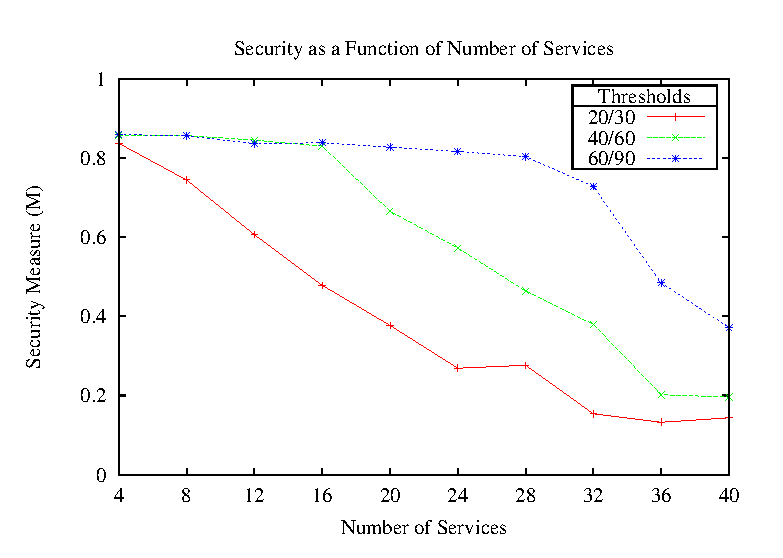
\includegraphics[width=0.5\textwidth]{num_services.eps}    
  \caption{Security as a Function of Number of Services}
    \label{fig:num_services}
\end{figure}

Figure \ref{fig:password_comp} considers the average password security measure ($M$) for the services as a function of the distribution of password composition policy strengths for two different cognitive parameter threshold pairs for reusing and writing down passwords respectively: 40/60 and 60/90. The notation (W,A,G,S) on the x-axis denotes the number of services that employ weak, average, good, and strong password composition policies. These results indicate that setting a password composition policy that optimizes password security may not be as obvious as one thinks. Requiring users to construct a stronger password may, in some cases actually worsen security. For example, the $M$ value for (0,32,0,0) was significantly higher than that for (0,0,32,0).

\begin{figure}
  \centering
  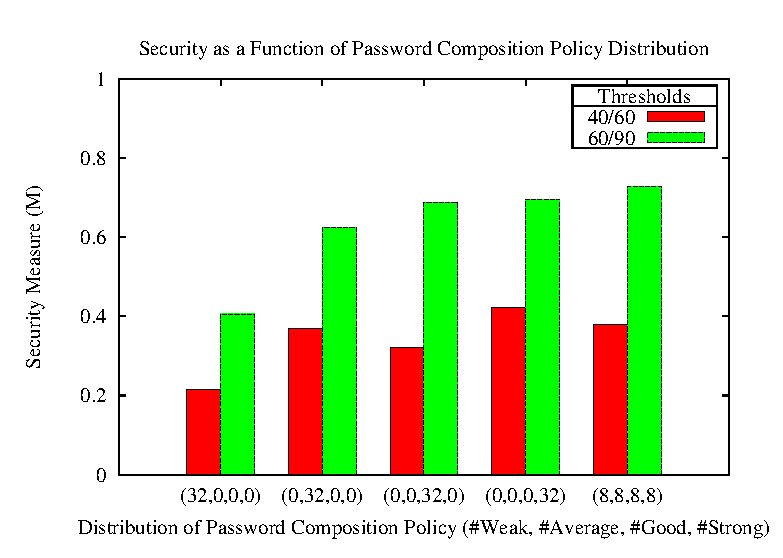
\includegraphics[width=0.5\textwidth]{password_comp.eps}    
  \caption{Security as a Function of Password Composition Policy Distribution}
  \label{fig:password_comp}  
\end{figure}

We reiterate that these results are only first steps and may be flawed. The model incorporates a number of unvalidated parameters such as weights for factors of $M$ that have tremendous influence on the outcomes of simulation runs. However, such graphs can still help in identifying issues with certain policy designs. A real-world environment is going to be even more nuanced so any surprises here will only become more pronounced. While we only make some simple observations here, with proper validation of these sorts of password models, one may be able to provide specific recommendations. Figure \ref{fig:num_services} tells us that we need to take into account the number of other services, the quality of those services, and user limitations in the design of password composition policies. Figure \ref{fig:password_comp} again reminds us that user cognitive limitations are an important factor in password security. Moreover, under certain assumptions regarding user memory, forcing users to create very strong passwords is ideal. But, in other situations, a mixture of weak, average, good, and strong passwords may actually improve overall security; Thus, having services collaborate in order to design password policy schemes may improve aggregate password security. 

\outlineedit{Suggested outline: short literature survey on
  passwords. 
  Well-known that there are cognitive limits on memory for passwords
that limits the number of complexity that individuals can remember. 

In addition, passwords are tied to a single-user access-to-all model
that doesn't work in many enterprises, so for example managers share
passwords with their admin assistants rather than employ circumscribed
but complex access control policies over the resources to be shared.

How do users create a more usable landscape for themselves? When
policies on password complexity are not enforced they are likely to be
ignored. When they are enforced, and particularly when used in
conjunction with a requirement to change a password after a certain
amount of time, two options are to store the password by some other
means, e.g. in physical writing, or to ``share'' passwords by using
the same or a very similar password between several sites. The
vulnerabilities caused by these workarounds depend on factors such as
how well protected is the physical copy and whether the password for a
high-value site is being shared with a site that is more vulnerable to
attack, perhaps because it is of low intrinsic value.
}

\outlineedit{
There are, then, a number of ways that user behavior may compromise
resources that are protected by passwords. We advocate a multi-agent
simulation to explore the dangers because the consequences of end user
action or of action taken by system administrators, such as
implementing password policies, are very difficult to model with a
statistical process. The number of vulnerabilities introduced by a
population of users cannot be predicted as an aggregate of independent
processes since users influence each other in a workplace. For
example, we have learned of cases where an admin found unencrypted
files of passwords on a number of user's computers that used the same
spreadsheet format, clearly indicating that the workaround had been
adopted from user to user and spread through their social network.
The consequences of the compromises depend on a complex array of
factors including the likelihood that a user uses a password that has
already been discovered by attackers on a high-value site.

The consequences of the defender's candidate actions are harder to
predict than those of an individual user. The defender may be faced
with the choice of requiring more complex passwords of all users, or
of enforcing a password lifetime. The danger to the defender's network
from each of these potential compromises depends on the compromised
user's access to sensitive data.

These factors indicate that a large-scale statistical approximation is
unlikely to provide a useful model of the potential effects of actions
taken by network defenders or end users. Instead we make use of
multi-agent models to explore the way that the defended system,
including computational elements and human actors, might respond to
alternative policy decisions. While our long-term aim with this work
is to estimate the expected value of alternative decisions under a
reasonable set of assumptions, in our initial work we show that our
simulation can reproduce some of the behaviors we have observed and
can highlight the sensitivity of the defender's best decision to a
number of factors as we describe below.

Modeling ideas coming from this: try modeling the effects of
  different policies with differing distributions in the population of
  cognitive limits and external site use and propensity to use bad
  workarounds, and finally different distributions of access to
  high-value resources and possibly social networks for sharing
  workarounds. For some of these, show how the profile of sensitivity
  to password policy changes.}

\section{Future Work}
\label{future_work}

While we feel there's a lot to be done in this space, primary foci for 
near-future work include adding to the password 
management model and building an agent-based model for an 
autologout scenario.

\subsection{Password Management Scenario}

We are interested in incorporating more faithful and/or better reasoned 
models and processes (e.g., \cite{florencio2014password})) for password 
recall, cognitive burden, and forgetfulness into our simulation. Once we've 
done this, we'd also like to revisit the work mentioned in this 
paper and explore other password management challenges. For a few examples, 
we'd like to (a) develop a more elaborate password simulation that 
incorporates communication and password sharing between users, exploring 
how group dynamics affect circumvention, (b) model how users cope with 
enterprise requirements requiring them to frequently reset their 
passwords, or (c) test alternative password policies (e.g., what would 
happen if we allowed users to write passwords on Post-It notes for a 
limited duration of time, but told them to rip up the Post-It notes afterward?). 
The idea of recognizing and even incorporating existing circumvention into 
the security model also seems like an interesting pursuit for modeling work. 
Last, while we have tried to validate our work with previous studies, this is 
an ongoing challenge and we would like to pursue new avenues and devise 
new experiments to aid on this front.

\subsection{The
  Auto-logout Scenario: the Effect of Security Policies on Group
  Behavior}
\label{auto-logout}

Tackling even an ostensibly simple problem, such as setting a 
``good''  timeout threshold, can be a nightmare in practice. As an 
example, consider the following anecdote. In a large hospital, 
clinicians frequently left shared computers logged-in but 
unattended \cite{kothari2014agent}.  Security officers, concerned 
about inappropriate access and inadvertent modification of patient 
data, opted to attach proximity sensors to the machines in an 
effort to mitigate these risks. These sensors detected when 
users had left terminals logged-in but unattended for some fixed 
timeout threshold. When such an event was detected, the 
logged-in user was automatically logged out of the machine. 
Clinician reception of these proximity sensors startled 
security officers.Clinicians, annoyed with the system, which was an 
impediment to doing actual work, placed styrofoam cups 
over the proximity sensors, which effectively tricked the proximity 
sensors into believing clinicians were nearby when they were not.
The proximity sensors were an absolute failure. Resources had 
been spent with the goal of improving security, but doing so yielded 
no security gains; instead, it was utterly defeated and it probably 
created a greater rift between clinicians and security personnel, 
making future security challenges even more difficult to address.

This anecdote highlights that it is essential to find solutions that 
make sense in the context of enterprise workflow-- solutions that 
can be successfully adopted by users whilst realizing security 
objectives without sabotaging other objectives.

So, how do we arrive at these solutions? It is usually impractical 
for security personnel to test out different security approaches 
within existing enterprises. Even if it is feasible, doing so often 
involves, at the minimum, substantial time, implementation costs, 
maintenance costs, and depletion of a finite user compliance 
budget \cite{beautement2009compliance}. We contend that 
multi-agent simulations may help distinguish good solutions 
from bad ones by predicting stress points of candidate 
implementations, thereby suggesting foci to improve upon. 
However, we are not suggesting that agent-based modeling is 
some magical panacea that can be used to address all security 
problems. It has its limits; it is nigh impossible to predict the 
unprecedented. Instead of trying to predict inventive workarounds 
such as the placement of styrofoam cups over proximity sensors, 
we aim to gauge user inclination to circumvent. 

In the case of auto-logouts, three main forces come into play. 
First, the use of shared workstations, in an environment where 
both users and systems are highly mobile, leads to the 
possibility of using another's credentials, inadvertently or not. 
Second, the nature of tasks, which involve prescribing 
medications and noting delivery, introduces potential risks 
for patient harm. Third, the frequency of leaving and returning 
coupled with the time spent logging in multiple times makes the 
auto-logout solution prohibitively burdensome.

Using simulation, we can explore the relevant factors that 
affect security risks associated with a clinician using a terminal to 
which another clinician is logged in. The likelihood of risk is 
affected by the number of agents, the number of workstations, 
group attitudes towards security and circumvention, and the 
dynamic nature of tasks; the actual risk is affected 
by the kinds of tasks performed. Simulations 
allow us to compare how burdensome different kinds of solutions 
are on users. For example, we might compare an auto-logout 
solution to a solution involving authentication challenges after a 
period of inactivity, which may slightly reduce the burden of 
having to log back in to a service; or, we could detect tasks that 
are disparate from the current task and warn the user that they 
may be using a terminal to which someone else is logged in. 
For some tasks, it may be possible to predict whether 
the worker must return to complete her session, and to apply 
different policies based on this prediction.

Last, while we mentioned the timeout problem in the medical 
setting, there are numerous other scenarios where auto-logouts 
may be relevant. And, we believe modeling approaches could 
be developed for them as well.

\section{conclusion}
\label{conclusion}

We have discussed our work toward building an agent-based model 
for a password management scenario. Though lacking in validation, 
we have made first steps and have generated graphs that led to 
interesting results. For example, we saw that our security measure 
is a function of the number of services with which the user engages. 
Additionally, under certain assumptions, making password composition 
more stringent may lead to a decrease in aggregate security. We contend 
that the agent-based modeling approach to addressing circumvention 
holds promise.

% An example of a floating figure using the graphicx package.
% Note that \label must occur AFTER (or within) \caption.
% For figures, \caption should occur after the \includegraphics.
% Note that IEEEtran v1.7 and later has special internal code that
% is designed to preserve the operation of \label within \caption
% even when the captionsoff option is in effect. However, because
% of issues like this, it may be the safest practice to put all your
% \label just after \caption rather than within \caption{}.
%
% Reminder: the "draftcls" or "draftclsnofoot", not "draft", class
% option should be used if it is desired that the figures are to be
% displayed while in draft mode.
%
%\begin{figure}[!t]
%\centering
%\includegraphics[width=2.5in]{myfigure}
% where an .eps filename suffix will be assumed under latex, 
% and a .pdf suffix will be assumed for pdflatex; or what has been declared
% via \DeclareGraphicsExtensions.
%\caption{Simulation Results}
%\label{fig_sim}
%\end{figure}

% Note that IEEE typically puts floats only at the top, even when this
% results in a large percentage of a column being occupied by floats.


% An example of a double column floating figure using two subfigures.
% (The subfig.sty package must be loaded for this to work.)
% The subfigure \label commands are set within each subfloat command, the
% \label for the overall figure must come after \caption.
% \hfil must be used as a separator to get equal spacing.
% The subfigure.sty package works much the same way, except \subfigure is
% used instead of \subfloat.
%
%\begin{figure*}[!t]
%\centerline{\subfloat[Case I]\includegraphics[width=2.5in]{subfigcase1}%
%\label{fig_first_case}}
%\hfil
%\subfloat[Case II]{\includegraphics[width=2.5in]{subfigcase2}%
%\label{fig_second_case}}}
%\caption{Simulation results}
%\label{fig_sim}
%\end{figure*}
%
% Note that often IEEE papers with subfigures do not employ subfigure
% captions (using the optional argument to \subfloat), but instead will
% reference/describe all of them (a), (b), etc., within the main caption.


% An example of a floating table. Note that, for IEEE style tables, the 
% \caption command should come BEFORE the table. Table text will default to
% \footnotesize as IEEE normally uses this smaller font for tables.
% The \label must come after \caption as always.
%
%\begin{table}[!t]
%% increase table row spacing, adjust to taste
%\renewcommand{\arraystretch}{1.3}
% if using array.sty, it might be a good idea to tweak the value of
% \extrarowheight as needed to properly center the text within the cells
%\caption{An Example of a Table}
%\label{table_example}
%\centering
%% Some packages, such as MDW tools, offer better commands for making tables
%% than the plain LaTeX2e tabular which is used here.
%\begin{tabular}{|c||c|}
%\hline
%One & Two\\
%\hline
%Three & Four\\
%\hline
%\end{tabular}
%\end{table}


% Note that IEEE does not put floats in the very first column - or typically
% anywhere on the first page for that matter. Also, in-text middle ("here")
% positioning is not used. Most IEEE journals/conferences use top floats
% exclusively. Note that, LaTeX2e, unlike IEEE journals/conferences, places
% footnotes above bottom floats. This can be corrected via the \fnbelowfloat
% command of the stfloats package.




% conference papers do not normally have an appendix


% use section* for acknowledgement
\section*{Acknowledgment}


This material is based in part upon work
supported by the Army Research Office
under Award No. W911NF-13-1-0086.






\nocite{*}

% trigger a \newpage just before the given reference
% number - used to balance the columns on the last page
% adjust value as needed - may need to be readjusted if
% the document is modified later
%\IEEEtriggeratref{8}
% The "triggered" command can be changed if desired:
%\IEEEtriggercmd{\enlargethispage{-5in}}

% references section

% can use a bibliography generated by BibTeX as a .bbl file
% BibTeX documentation can be easily obtained at:
% http://www.ctan.org/tex-archive/biblio/bibtex/contrib/doc/
% The IEEEtran BibTeX style support page is at:
% http://www.michaelshell.org/tex/ieeetran/bibtex/
\bibliographystyle{IEEEtran}
% argument is your BibTeX string definitions and bibliography database(s)
%\bibliography{IEEEabrv,../bib/paper}
\bibliography{refs}
%
% <OR> manually copy in the resultant .bbl file
% set second argument of \begin to the number of references
% (used to reserve space for the reference number labels box)

%\begin{thebibliography}{1}
%
%\bibitem{IEEEhowto:kopka}
%H.~Kopka and P.~W. Daly, \emph{A Guide to \LaTeX}, 3rd~ed.\hskip 1em plus
%  0.5em minus 0.4em\relax Harlow, England: Addison-Wesley, 1999.
%
%\end{thebibliography}


% that's all folks
\end{document}


